%# -*- coding: utf-8-unix -*-
%%==================================================


\chapter{波动光学}
\label{chap2}



\section{干涉}



\subsection{杨氏双缝及其变形}
\begin{myprop}{ 经典杨氏双缝}{}
    当一束光经过两个相距为$d$($d$很小)的小孔之后,在距离小孔为$D$的干涉屏上出现干涉条纹,其间距为
    \[
        \Delta x=\dfrac{D}{d}\lambda
    \]
\end{myprop}
从公式上看,相当于把波长放大$\dfrac{D}{d}$倍,这是一种最典型的\textbf{分波前}干涉的方法。


\begin{myprop}{杨氏双缝变形}{1}
	
	各种杨氏双缝变式本质上也是两个点光源进行干涉,只是前者更加直接
	\[
		\begin{tabular}{ccc}
			\hline 干涉名称 & 等效 $d$ & 等效 $D$ \\
			\hline 双棱镜 & 虚光源距离 $2 s_1(n-1) \alpha$ & 虚光源与干涉平面的间距 $s_1+s_2$ \\
			劳埃镜 & 光源与镜面像距离 $2 d$ & 光源与干涉平面的间距 $D$ \\
			对切透镜 & 两个半透镜成像距离 $2 y^{\prime}$ & 成像平面与干涉平面的间距 $L-v$ \\
			\hline
		\end{tabular}
	\]
\end{myprop}

以上都是将光束分成两束不同的子波进行干涉,都属于\textbf{分波前干涉},还有一种干涉类型为\textbf{分振幅干涉}。

\begin{mydef}{干涉类型}{1}
	\begin{itemize}
		\item \textbf{分波前法}:让光波通过并排的两个小孔或利用反射和折射方法, 把光波的波前分割出两个部分(本质上是\textbf{惠更斯原理}),形成两个次波重新叠加发生干涉;
		\item \textbf{分振幅法}:利用光在介质表面分割产生两个反射光或两透射光波(反射和透射如何分配,本质上是\textbf{菲涅尔衍射公式}),两者走过不同的光程,重新叠加并发生干涉。
	\end{itemize}
\end{mydef}
\subsection{薄膜干涉和迈克尔逊干涉仪}

\begin{myprop}{ 等厚干涉光程差}{1}
	一束光从空气射入厚度为$h$的薄膜,其折射角为$i$,则该束光在薄膜上下反射的两束光光程差为
	\[
		\Delta = 2nh\cos i
	\]
\end{myprop}
\begin{figure}[htbp]
	\centering
	\includegraphics[width=5.5cm]{fig12.eps}
	\caption{等厚干涉光路图}
\end{figure}
\begin{proof}
	由折射定律$\sin r=n\sin i$,而上束光多走了$x_1=h\cdot 2\tan i\cdot \sin r$,下束光多走了$x_2=n\cdot \dfrac{2h}{\cos i}$,则光程差计算为
	\[
		\begin{aligned}
			\Delta&=\dfrac{2nh}{\cos i}-2h\tan i\sin r=2h(\dfrac{n}{\cos i}-\dfrac{\sin i \cdot \textcolor{blue}{\sin r}}{\cos i})\\
			&=2h(\dfrac{n}{\cos i}-\dfrac{\sin i \cdot \textcolor{blue}{n \sin i}}{\cos i})
			=2nh\dfrac{1-\sin^2 i}{\cos i}=2nh\cos i
		\end{aligned}
	\]
\end{proof}
\begin{myprop}{ 迈克尔逊干涉仪光程差}{1}
	迈克尔逊干涉仪的结构类似“麻将”局,东西南北方都要经过,其光程差为长度差的两倍
	\[
		\Delta=2(l_1-l_2)
	\]
\end{myprop}

% \subsection{相干性}
% \begin{itemize}
% 	\item 时间相干性
% 	\item 空间相干性
% \end{itemize}


\section{衍射}

\begin{itemize}
	\item \textbf{菲涅尔衍射(近场衍射)}:光源或观察屏到衍射屏的距离为\textbf{有限}的衍射。
	\item \textbf{夫琅禾费衍射(远场衍射)}:光源和观察屏到衍射屏的距离均为\textbf{无限}的衍射。
\end{itemize}


\subsection{半波带法}
\begin{itemize}
	\item \textbf{夫琅禾费单缝衍射的半波带法}
\end{itemize}
\quad \quad 把单缝分割成一系列条带, 相邻条带之间的光程逐个相差半个波长, 称为半波带。
	相邻半波带贡献的复振幅相位差为$\pi$,在图示中表现为相邻矢量,$A_k$和$A_{k+1}$向。
	容易知道,每条半波带的贡献相等,不妨记作$A_1=A_2=\cdots=A_k=A$
	\par 当半波带总数为奇数时,$A_{total}=A$,偶数时,$A_{total}=0$
\begin{figure}[!htp]
	\centering
	\includegraphics[width=4.5cm]{fig1.png}
	\hspace{1cm}
	\includegraphics[width=4.5cm]{fig2.png}
	\caption{夫琅禾费单缝衍射的半波带法图例}
\end{figure}

\begin{itemize} 
	\item \textbf{菲涅尔圆孔衍射的半波带法}
\end{itemize}

\par 波前分割为一系列环形带,相邻环形带到像点的距离逐个相差半个波长,称为半波带。相邻半波带贡献的复振幅相位差为$\pi$,在图示中表现为相邻矢量$A_k$,和$A_{k+1}$反向。
\par 不同于单缝衍射,由于倾斜因子影响,每条半波带的贡献,逐渐减小$\displaystyle \lim_{k\rightarrow \infty}A_{K}=0$
\begin{figure}[!htp]
	\centering
	\includegraphics[width=4.5cm]{fig3.png}
	\hspace{1cm}
	\includegraphics[width=4.5cm]{fig4.png}
	\caption{菲涅尔圆孔衍射的半波带法图例}
\end{figure}
\newline


\begin{myprop}{菲涅尔波带片}{}
	\[
	\frac{1}{R}+\frac{1}{b}=\frac{k \lambda}{\rho_k^2}
	\]
	当物距 $R$, 像距 $b$ 时 $\left[\begin{array}{c}1 \text {. 通过 } \rho_k \text { 的光线 } \\ 2 \text {. 通过 } \rho_0=0 \text { 的光线(与光轴重合的光线) }\end{array}\right]$ 光程差为 $k \lambda$
\end{myprop}

\begin{example}
	单色平面光波波长 \qty{5000}{\angstrom},正入射到如下图所示的衍射屏上,$r_1=\sqrt{2} \mathrm{~mm}$, $r_2=1 \mathrm{~mm}$,轴上观察点离衍射屏 $2 \mathrm{~m}$,计算观察点处的振幅和强度 (用$A_0$和$I_{0}$ 表示) 。
	\soln

	\[
		\\
	\]
	\[
		\\
	\]
	
	% \par 由波带片计算相应的半波带数目
	% \[
	% 	k_{i}=\dfrac{\rho_i^2(R+b)}{Rb}=2,1	
	% \]
	% \par 图中相当于一个完整$k\in[0,1]$半波带和$\dfrac{1}{4}$个$k\in[1,2]$半波带,绘制相应矢量振幅图如下,从图中可得
	% \[
	% 	A_{合}=1.5A_0,I_{合}=2.25I_0	
	% \]
\end{example}

\begin{figure}[!htp]
	\centering
	\subcaptionbox{例2.4题图}[4cm]
	{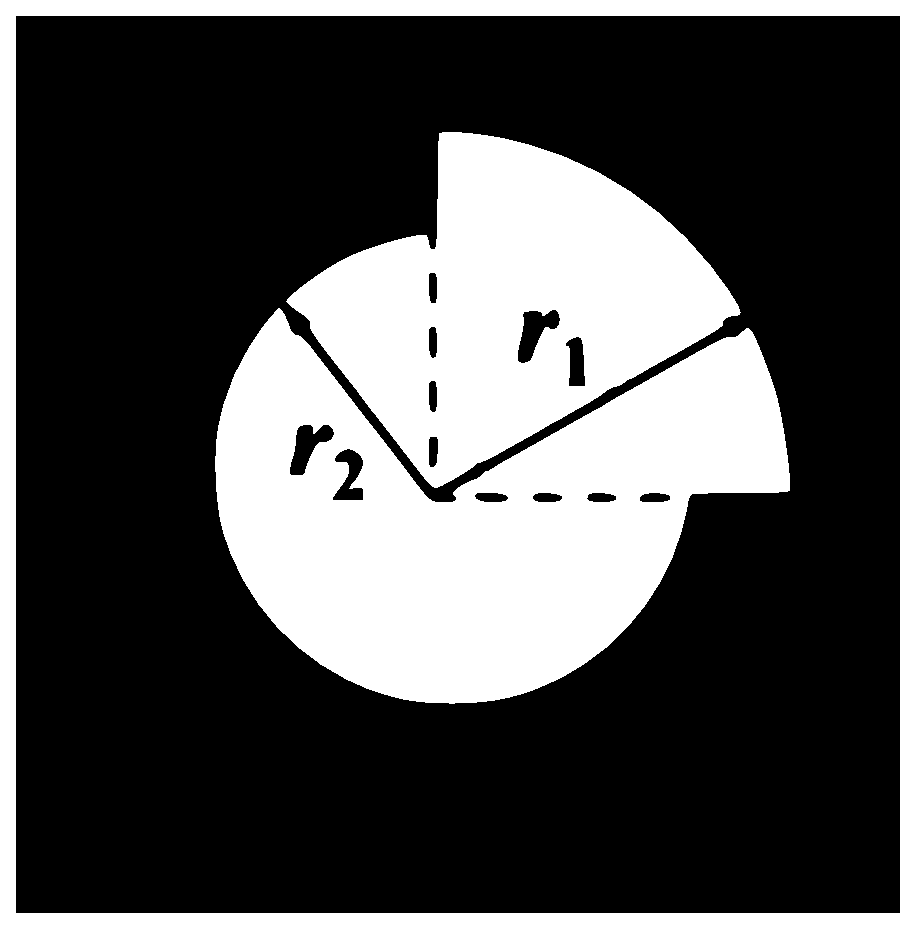
\includegraphics[width=4cm]{fig8.eps}}
	% \hspace{1cm}
	% \subcaptionbox{例2.4矢量分析图}[7cm]
	% {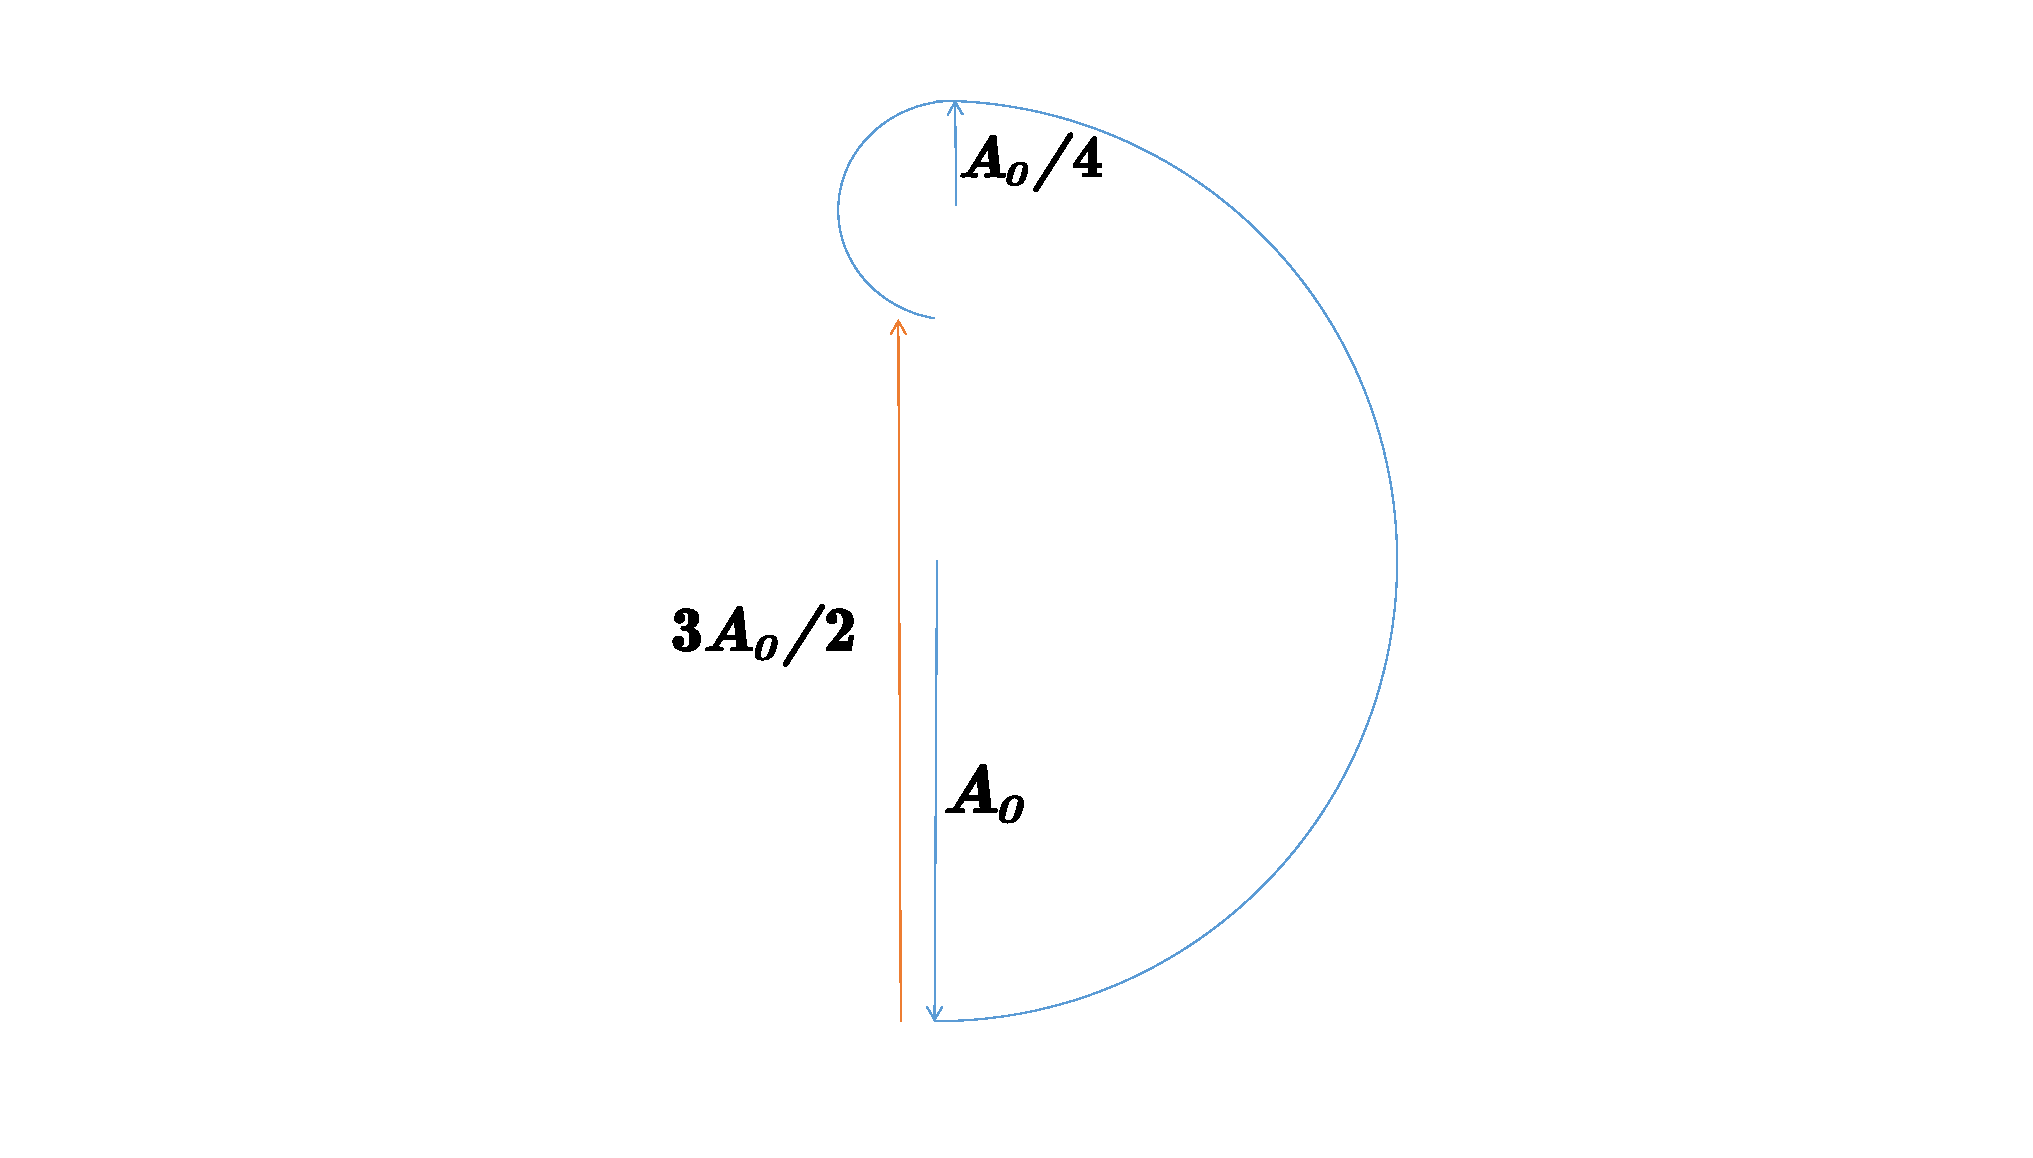
\includegraphics[width=8cm]{fig11.eps}}
	\caption{半波带法的具体例子}
\end{figure}

\subsection{振幅矢量法}
\begin{itemize}
	\item \textbf{夫琅禾费单缝衍射的振幅矢量法}
\end{itemize}
\par 振幅矢量法不要求 $\sin \varphi=k \dfrac{\lambda}{2}$,可以视作半波带法的细化 $i . e$. 普适版本。 具体说来,它将单缝分割成 $d x \rightarrow 0$ 的微元,相位差 $d \theta=\dfrac{2 \pi}{\lambda} d x \sin \varphi$,于是总相位差
\[
	\cancel{\begin{array}{c}
		2\\
	\end{array}}\alpha =\frac{\cancel{2}\pi}{\lambda}a\sin \varphi 
\]
\par 因此, 若将 $\varphi=0 \equiv \theta$ 时的振幅记作 $A_0$, 从而绘制矢量图得到
\begin{figure}[!htp]
	\centering
	\includegraphics[width=4.5cm]{fig5.png}
	\caption{光栅振幅矢量法图例}
\end{figure}
\begin{myprop}{ 单缝衍射因子}{}
	在单缝衍射中,定义$\alpha=\dfrac{\pi a\sin \theta}{\lambda}$,则振幅和光强分布如下
	\[
		A_{\varphi}=\left(\frac{\sin \alpha}{\alpha}\right) A_0 \Rightarrow I_{\theta}=\left(\frac{\sin \alpha}{\alpha}\right)^2 I_0
	\]
\end{myprop}

\begin{itemize} 
	\item \textbf{菲涅尔圆孔衍射的振幅矢量法}
\end{itemize}
\begin{mythm}{菲涅尔衍射公式}{2}
	\[
		\widetilde{U}(P)=K\iint_{\Sigma}{F\left( \theta _0,\theta \right) \frac{e^{ikr}}{r}\widetilde{U_0}(Q)\mathrm{d}\Sigma}
	\]
	\[
	F: \text{倾斜因子} \quad   \frac{e^{ikr}}{r}: \text{距离因子}\quad  \widetilde{U_0}(Q) \mathrm{d}\Sigma : \text{次波源强度}
	\]
\end{mythm}
\par 当 $\Sigma$ 代表点波源产生的球面波波前,$\widetilde{U_0}(Q)$ 为常量,$\dfrac{\mathrm{d} \Sigma}{r} \propto \mathrm{d} r$,故上式可写作
\[
\widetilde{U}(P)=C \int_{\Sigma} e^{i k\left(r-r_0\right)} F\left(\theta_0,\theta\right) \mathrm{d} r
\]
\par 由于 $r$ 变化时 $e^{i k\left(r-r_0\right)}$ 变化较快,$F\left(\theta_0,\theta\right)$ 变化较慢,所以我们先忽略 $F\left(\theta_0,\theta\right)$ 的变化,此时
\[
\widetilde{U}(P)=C^{\prime} \int_{\Sigma} e^{i k\left(r-r_0\right)} \mathrm{d} r
\]
\par 这一积分可以用复平面上的矢量图来表示。
\par

\par 至此, 与夫琅禾费单缝衍射的振幅矢量法别无二致。接下来考虑倾斜因子, 随着 $r$ 的增大 $i.e$.
倾角的增倾斜因子 $F \rightarrow 0$,于是图中半径 $R \rightarrow 0$,形成菲涅尔螺线。 可以发现 若将每个半圆用其直径来代替, 则退化成半波带法。


使用\verb+siunitx+宏包可以方便地输入SI单位制单位,例如\verb+\SI{5}{\um}+可以得到\SI{5}{\um}。

\subsection{多缝干涉和艾里斑}
若光栅缝间距为 $d$, 则缝间相位差
$$
\not{2} \beta=\delta=\frac{\not 2 \pi}{\lambda} d \sin \varphi
$$
Thus, 若将单缝振幅记作 $A_1$, 矢量图如下
\begin{figure}[!htp]
	\centering
	\includegraphics[width=4.5cm]{fig6.png}
	\caption{菲涅尔圆孔衍射的振幅矢量法图例}
\end{figure}
$$
A_{\varphi}=\left(\frac{\sin N \beta}{\sin \beta}\right) A_1 \Rightarrow I_{\varphi}=\left(\frac{\sin N \beta}{\sin \beta}\right)^2 I_1
$$
这正是光栅的缝间干涉因子。于是
\begin{myprop}{ 光栅衍射因子}{}
	在光栅衍射中,定义$\alpha=\dfrac{\pi a\sin \varphi}{\lambda},\beta=\dfrac{\pi d\sin \varphi}{\lambda}$,则振幅和光强分布如下
	\[
		A_{\varphi}=\left(\frac{\sin N \beta}{\sin \beta}\right)\left(\frac{\sin \alpha}{\alpha}\right) A_0 \Rightarrow I_{\varphi}=\left(\frac{\sin N \beta}{\sin \beta}\right)^2\left(\frac{\sin \alpha}{\alpha}\right)^2 I_0
	\]
\end{myprop}

\begin{mydef}{光栅本领}{2}
	\begin{itemize} 
	\item $k$ 级主极大条件: $\beta_k=k \pi \Leftrightarrow d \sin \varphi_k=k \lambda\left(\right.$ (微分 : $\left.d \cos \varphi_k \delta \varphi_k=\delta(k \lambda)\right)$
	\item $k$ 级主极大半角宽: $\Delta \beta_k=\dfrac{\pi}{N} \Leftrightarrow d \cos \varphi_k \Delta \varphi_k=\dfrac{\lambda}{N} \Leftrightarrow \Delta \varphi_k=\dfrac{\lambda}{N d \cos \varphi_k}$
	\item  分辨本领 : $d \sin \left(\varphi_k \pm \Delta \varphi_k\right)=k(\lambda \pm \delta \lambda) \Leftrightarrow d \cos \varphi_k \Delta \varphi_k=k \delta \lambda=\dfrac{\lambda}{N} \Leftrightarrow R=\dfrac{\lambda}{\delta \lambda}=k$
	\item  角色散本领 $: D_\theta \equiv \dfrac{\delta \varphi_k}{\delta \lambda}=\dfrac{k}{d \cos \theta_k}$
	\item  线色散本领 $: D_l=f \cdot D_\theta=\dfrac{k f}{d \cos \theta_k}$
	\end{itemize}
\end{mydef}

\begin{example}
	一个三狭缝衍射屏, 缝宽均为 $\boldsymbol{a}$, 彼此间距为 $\boldsymbol{d}$, 中间缝盖有可以引起 $180^{\circ}$ 相位改变的滤光片, 波长为 $\lambda$ 的单色光正人射, 计算下列各种情况下 的衍射角:
	\par (1) 第一衍射极小;
	\par (2) 第一干涉极小;
	\par (3) 第一干涉极大。
	\soln

	\[
		\\
	\]
	\[
		\\
	\]
	\[
		\\
	\]
	% \par (1)定义$\alpha=\dfrac{\pi a\sin \theta}{\lambda}$,则单缝衍射因子为$\left(\dfrac{\sin \alpha}{\alpha}\right)^2$,则第一衍射极小对应的角度$\alpha=\pi$,解得
	% \[
	% 	\dfrac{\pi a\sin \theta_1}{\lambda}=\pi\Longrightarrow \theta_{1}=\dfrac{\lambda}{a}	
	% \]
	% \par (2)由于对称性,将中心缝作为基准,则定义$\delta=\dfrac{\textcolor{blue}{2}\pi d\sin \theta}{\lambda}$为相邻两束光干涉的相位差,其振幅合成大小为
	% \[
	% 	A_{合}=A_{0}(2\cos \delta-1)	
	% \]
	% \par 当$A=0$时,绝对值最小的解为$\delta=\pm \dfrac{\pi}{3}$,则
	% \[
	% 	\dfrac{\textcolor{blue}{2}\pi d \sin \theta_2}{\lambda}=\dfrac{\pi}{3}\Longrightarrow\theta_2=\dfrac{\lambda}{6d}
	% \]
	% \par (3)干涉极大对应$|2\cos \delta -1|$极大,此时$\delta=\pm \pi$,则
	% \[
	% 	\dfrac{\textcolor{blue}{2}\pi d \sin \theta_3}{\lambda}=\pi\Longrightarrow\theta_3=\dfrac{\lambda}{2d}	
	% \]
\end{example}

% \begin{figure}[!htp]
% 	\centering
% 	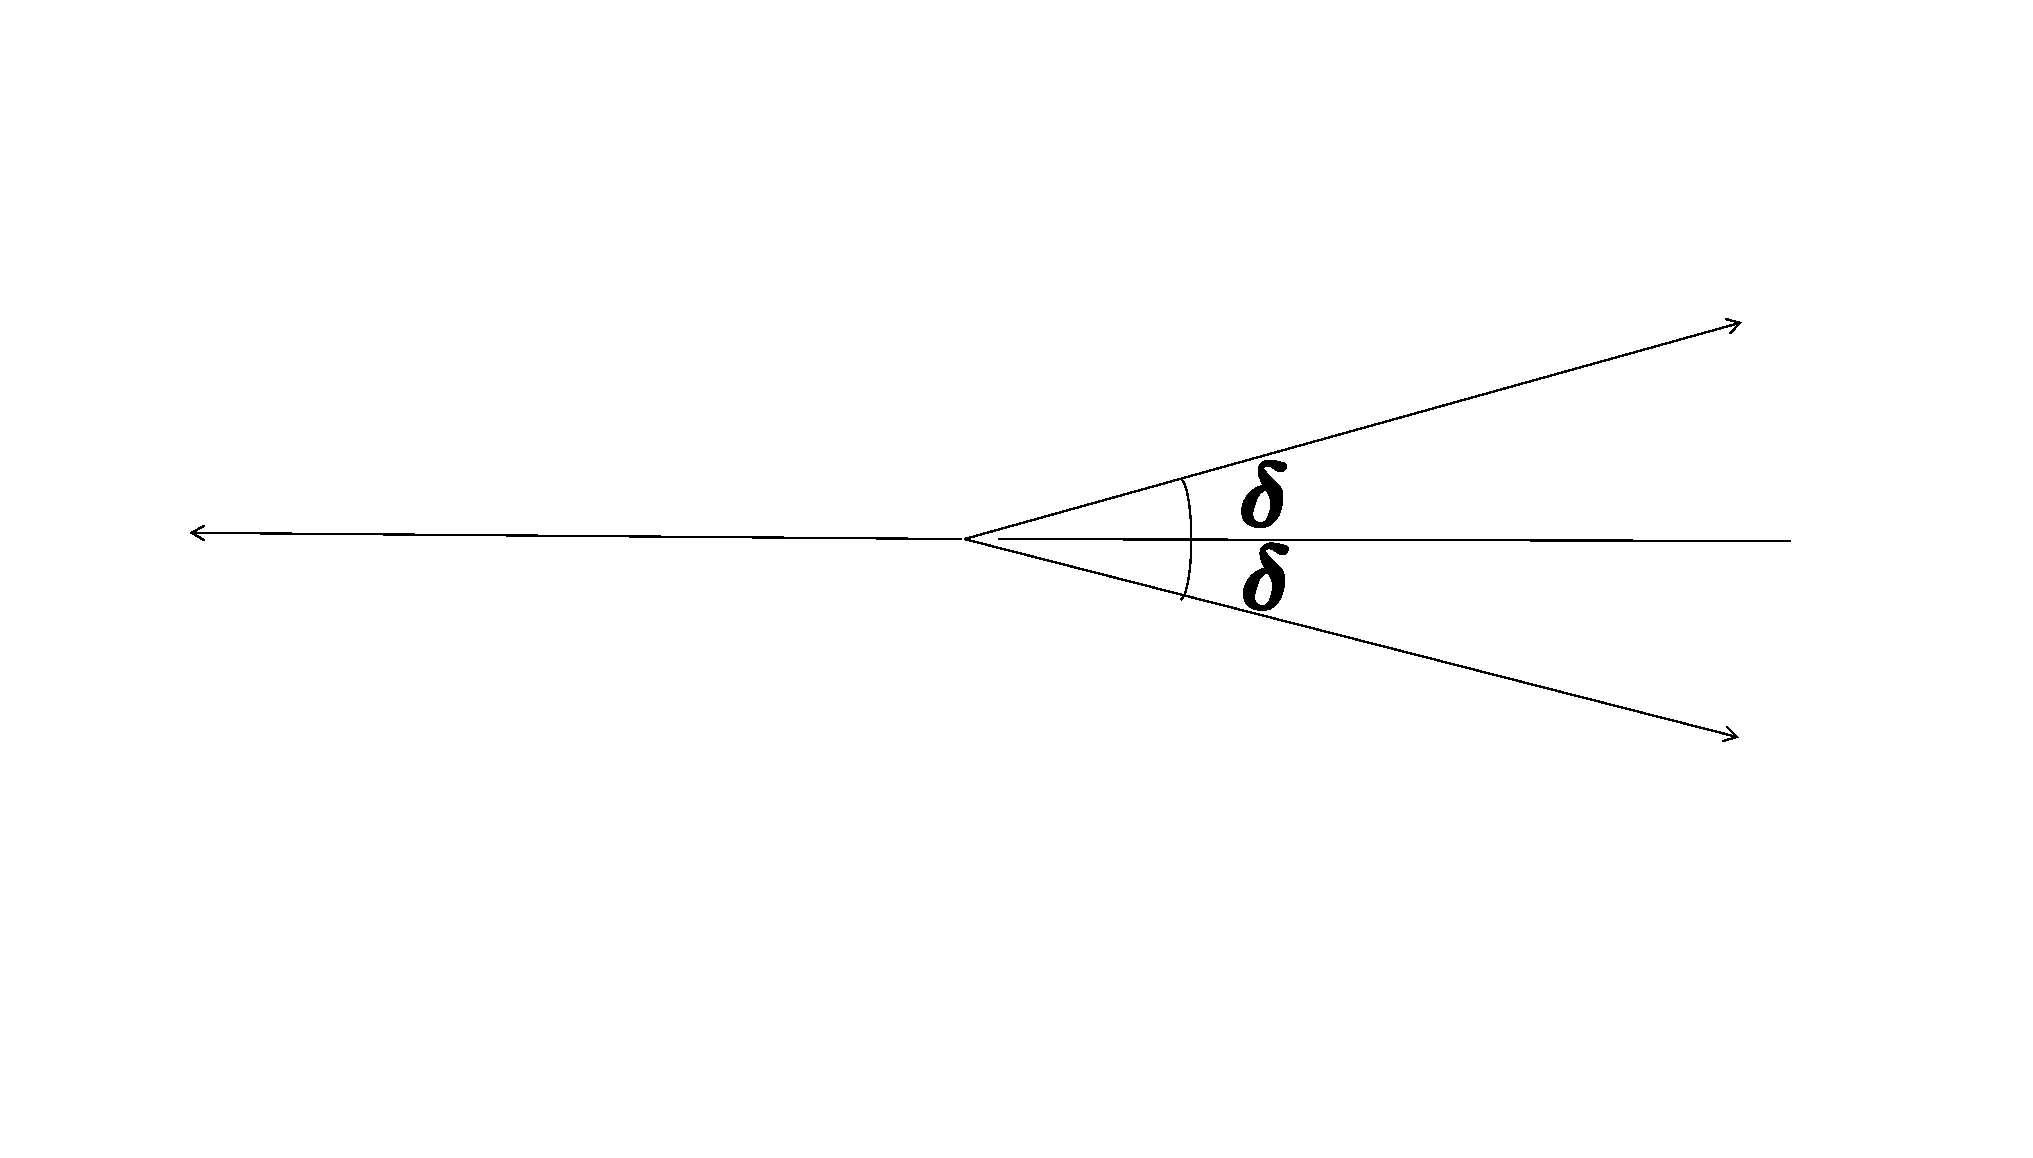
\includegraphics[width=8cm]{fig10.eps}
% 	\caption{例2.8 光栅振幅矢量法图例}
% \end{figure}
\begin{myprop}{艾里斑}{1}
	艾里斑是点光源通过理想透镜成像时,由于绕射而在焦点处形成的光斑,其最小分辨角以及分辨本领分别公式为:
	\[
		\delta \theta=\theta_1 \approx 1.22 \frac{\lambda}{D},R \equiv \frac{1}{\delta \theta}=\frac{D}{1.22 \lambda}
	\]
\end{myprop}
\begin{figure}[!htp]
	\centering
	\includegraphics[width=5cm]{fig7.png}
	\caption{艾里斑示意图}
\end{figure}








\section{偏振}

\subsection{菲涅尔反射折射公式}

斯托克斯公式、两个光路图推导
公式定性推导、半波损失、全反射、隐失波的解释

\begin{myprop}{斯托克斯倒逆关系}{1}
如下图所示,设光从介质A传播到介质B的反射系数和透射系数分别为$r,t$,从介质B到介质A的反射系数和透射为$r^{\prime},t^{\prime}$,以下关系式成立(四个系数均为复数)
	\[
		\left\{\begin{array}{l}r^{\prime}=-r \\ r^2+t t^{\prime}=1\end{array}\right.
	\]
\end{myprop}
\begin{proof}
	如图所示,由于光路可逆,将反射光和透射光按照原路照射返回,对应振幅不变即可。
\end{proof}
\begin{figure}[!htp]
	\centering
	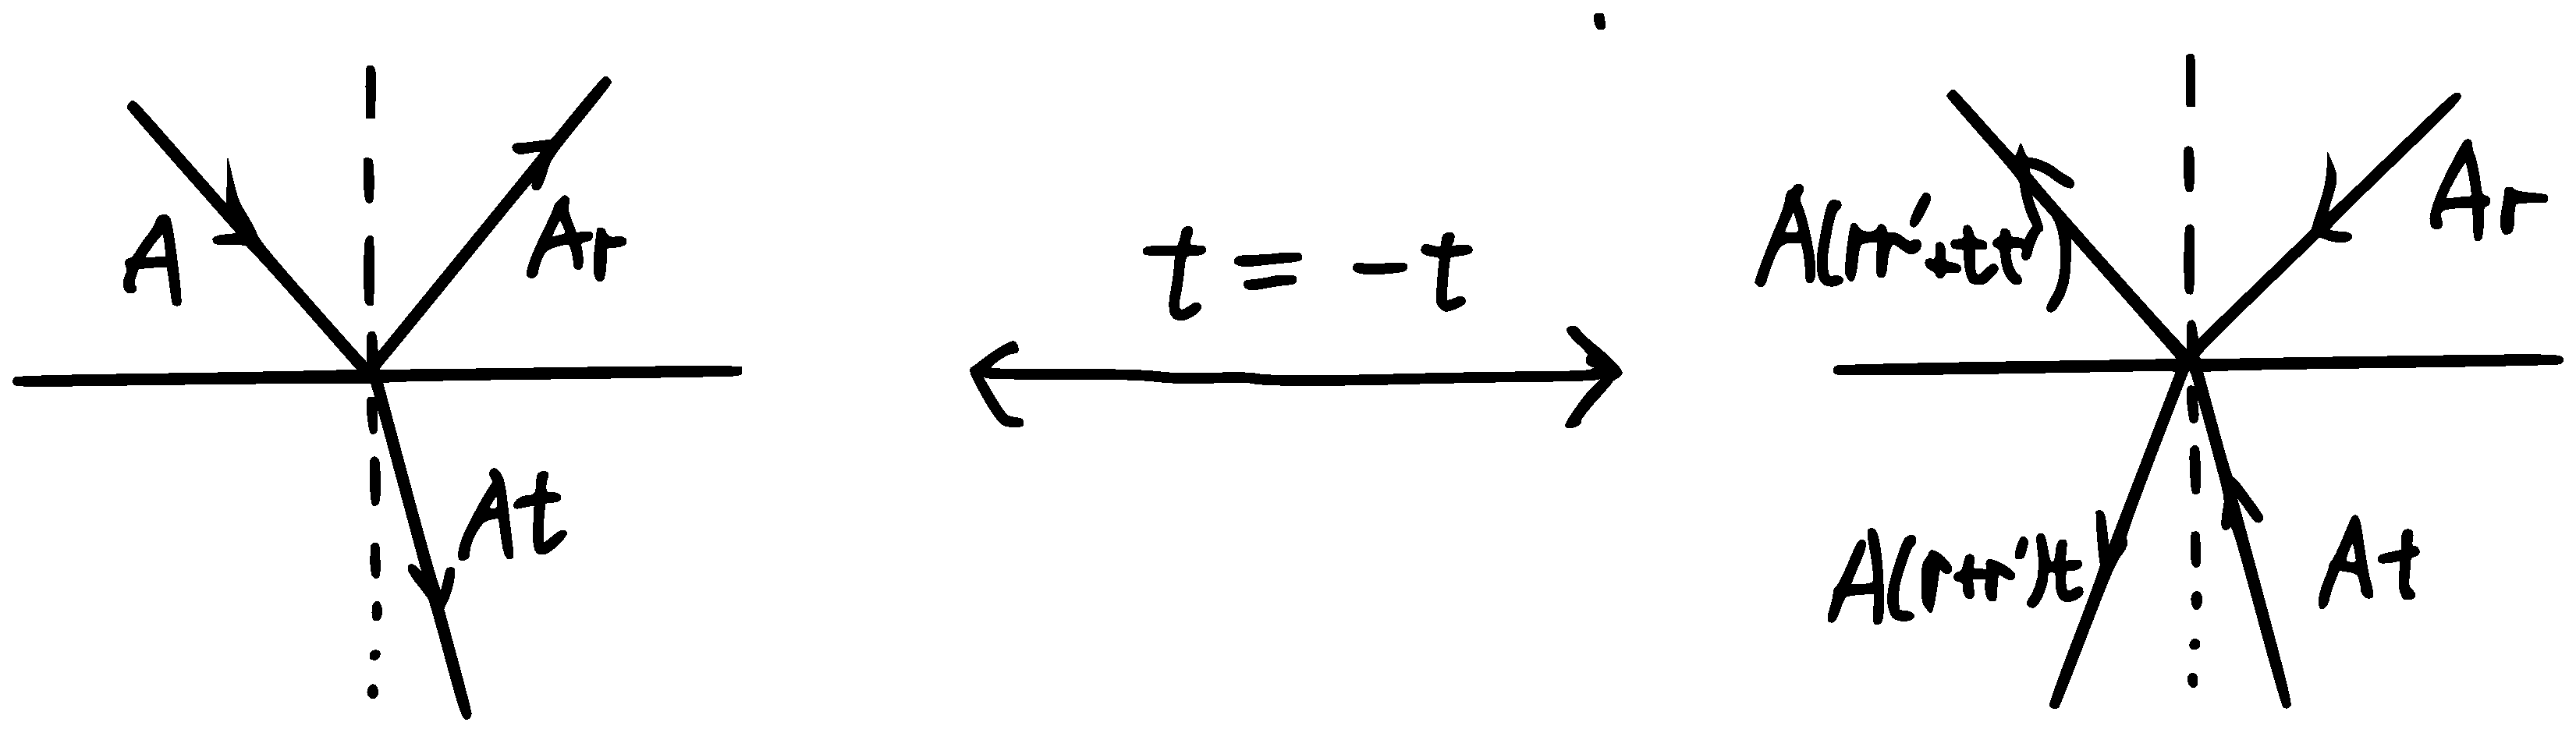
\includegraphics[width=12cm]{fig13.eps}
	\caption{斯托克斯倒逆关系示意图}
\end{figure}

\begin{myprop}{菲涅尔公式}{1}
	光在两种不同折射率的介质中传播时,其反射光和折射光在垂直平面和平行平面分量($p$光和$s$光)对应系数如下:
		\[
			\left\{\begin{array}{l}
				r_s=\dfrac{n_1 \cos i_1-n_2 \cos i_2}{n_1 \cos i_1+n_2 \cos i_2} \quad t_s=\dfrac{2 n_1 \cos i_1}{n_1 \cos i_1+n_2 \cos i_2} \\
				r_p=\dfrac{n_2 \cos i_1-n_1 \cos i_2}{n_1 \cos i_2+n_2 \cos i_1} \quad t_p=\dfrac{2 n_1 \cos i_1}{n_1 \cos i_2+n_2 \cos i_1}
				\end{array}\right.
		\]
\end{myprop}
\begin{figure}[!htp]
	\centering
	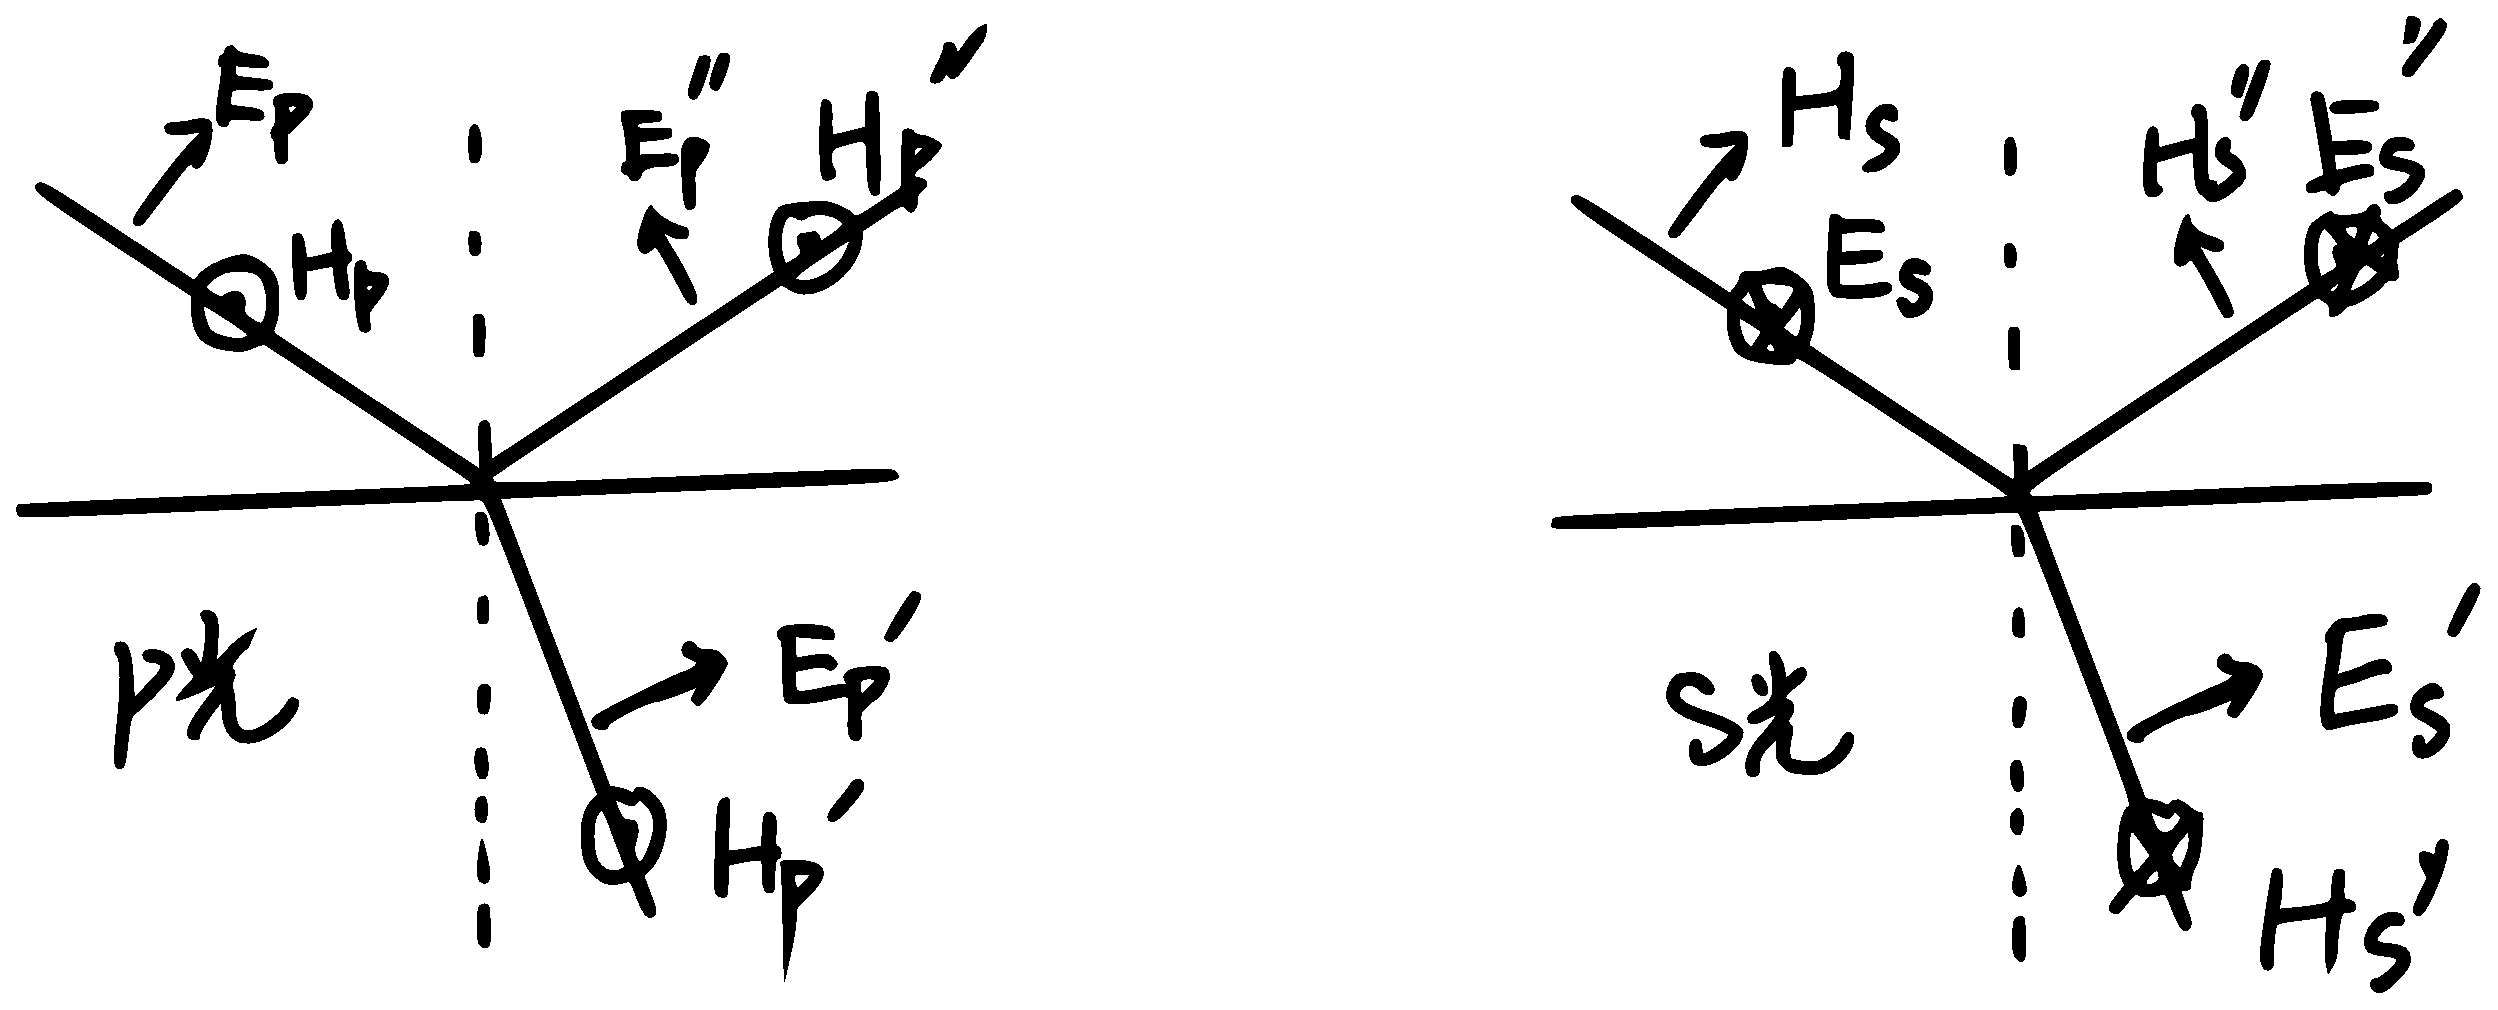
\includegraphics[width=10cm]{fig14.eps}
	\caption{菲涅尔公式示意图}
\end{figure}

\begin{proof}
	该公式推导需要运用到电磁场的边界条件,此处从略,可点击\href{https://zhuanlan.zhihu.com/p/520141099}{此链接}查看。
\end{proof}


\begin{myprop}{ 正入射情形}{1}
	当$i_1=i_2=0$时,$n_2>n_1$
	\[
		\begin{aligned}
			&r_s<0,\ E_{s}^{\prime\prime}\text{与}E_{s}\text{正方向相同}\\
			&r_p>0,\ E_{p}^{\prime \prime}\text{与}E_{p}\text{正方向相反,产生严格的半波损失}
		\end{aligned}
	\]
\end{myprop}

\begin{remark}
	《光学》教材对于全反射情况下相位变化公式推导缺少负号(见下),本质上是求复数幅角$\arg\dfrac{A-Bi}{A+Bi}=-2\arctan\left(\dfrac{B}{A}\right)$
	\[
	\begin{array}{l}\delta_{\mathrm{p}}=\textcolor{blue}{-}2 \arctan \dfrac{n_1}{n_2} \dfrac{\sqrt{\left(\dfrac{n_1}{n_2}\right)^2 \sin ^2 i_1-1}}{\cos i_1}, \delta_{\mathrm{s}}=\textcolor{blue}{-}2 \arctan \dfrac{n_2}{n_1} \dfrac{\sqrt{\left(\dfrac{n_1}{n_2}\right)^2 \sin ^2 i_1-1}}{\cos i_1} .\end{array}
	\]
\end{remark}

\begin{example}
	$s$光以$\theta$角从折射率$n_1$介质入射厚度为$d$、折射率为$n_2$的玻璃平板后回到$n_1$介质($n_2>n_1$),求以下两种情况的能量透射率:
	\par (1)\ $d$很小,相邻出射光束间仍有相干性;
	\par (2)\ $d$很大,相邻出射光束间无相干性。(提示:类比法布里-珀罗干涉仪)
	\soln

	\[
		\\
	\]
	\[
		\\
	\]
	\[
		\\
	\]
\end{example}


\subsection{双折射和$\dfrac{\lambda}{4}$片}
\begin{myprop}{ 光学介质}{1}
	如下图所示,规定主截面为法线和光轴所在平面,o光为偏振方向垂直主截面,e光为偏振方向平行主截面:
\end{myprop}
\begin{figure}[!htp]
	\centering
	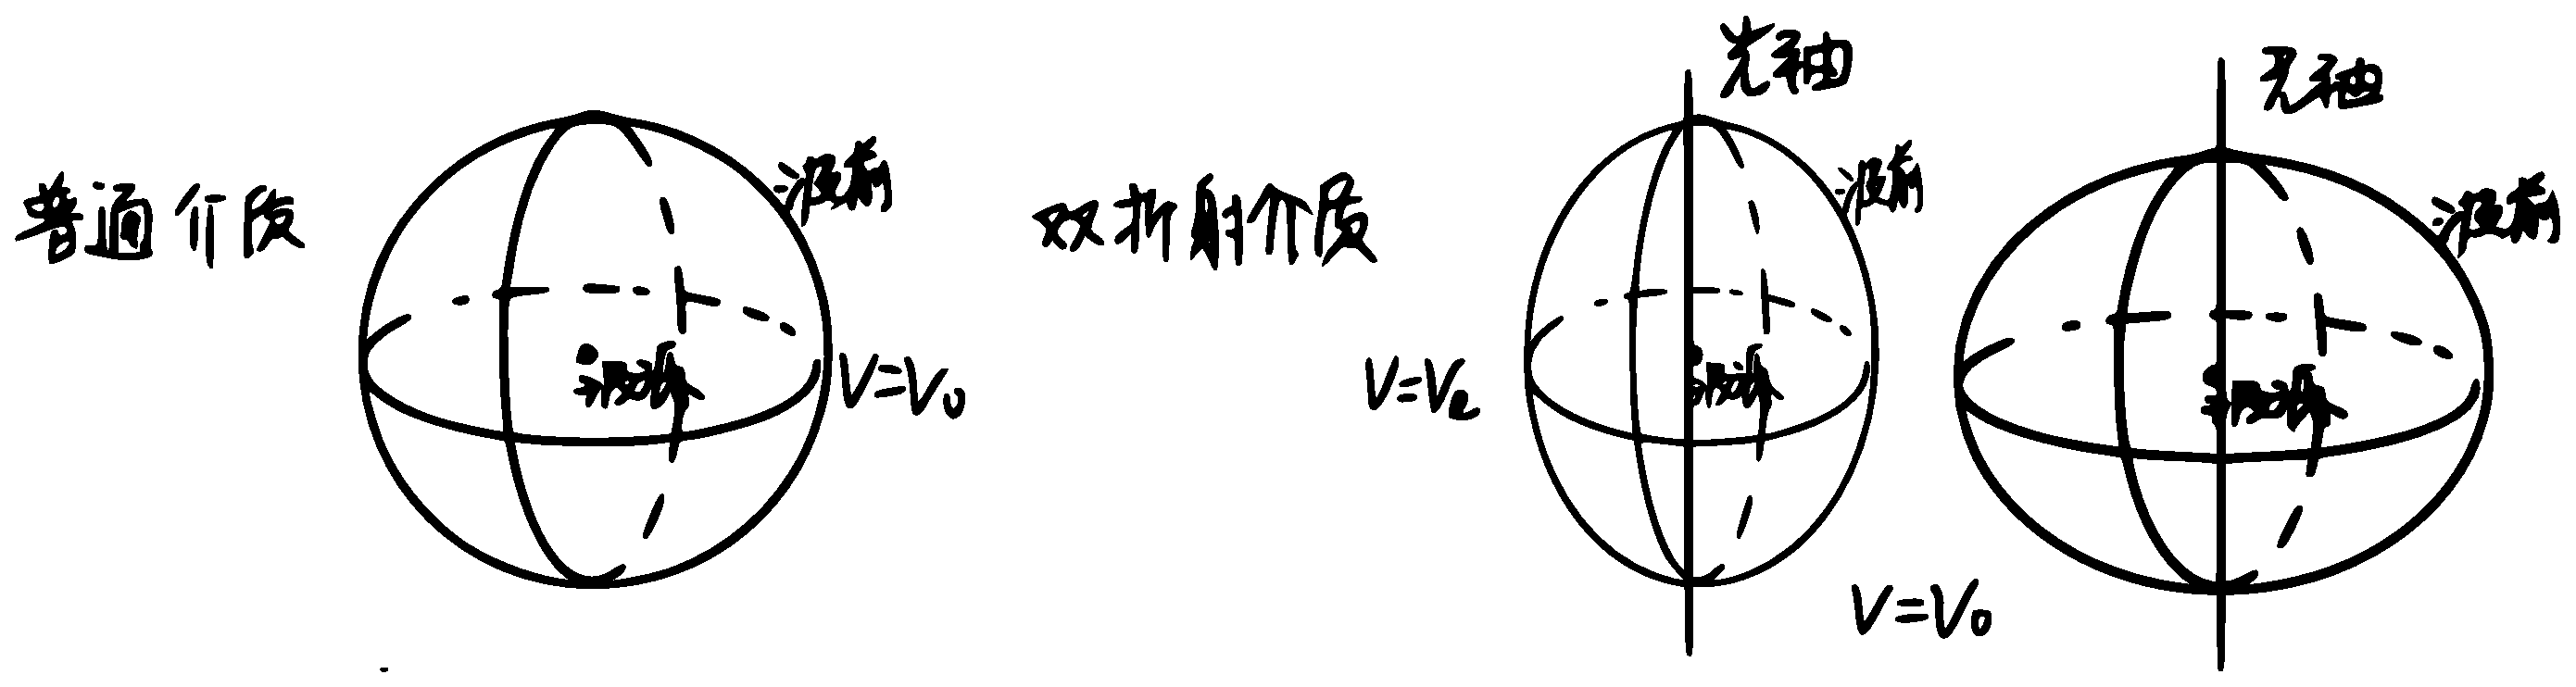
\includegraphics[width=11cm]{fig15.eps}
	\caption{普通介质和光学介质示意图}
\end{figure}
\begin{example}
	求以下两种情况的折射角$r$和波矢与法线夹角$\theta$(入射光在主截面内)
	\par \ (1)入射角为$i$,光轴平行法线;
	\par \ (2)入射光平行法线,光轴与法线夹角为$\varphi$。
	\soln

	\[
		\\
	\]
	\[
		\\
	\]
	\[
		\\
	\]
\end{example}
\begin{myprop}{ 双折射应用}{1}
	以下三种棱镜均使用了$o$光和$e$光双折射性质:
\end{myprop}
\begin{figure}[!htp]
	\centering
	\includegraphics[width=11cm]{fig16.png}
	\caption{Rochon棱镜、Wolluston棱镜、Nicol棱镜示意图}
\end{figure}

\begin{myprop}{ $\dfrac{\lambda}{4}$片}{1}
	对下图所示波晶片, $o$ 光、 $e$ 光在通过波晶片后产生相位差,其满足
	\[
		\Delta=\frac{2 \pi}{\lambda}\left(n_o-n_e\right) d	
	\]
	当 $\left(n_o-n_e\right) d=\dfrac{\lambda}{4}$ 时,$\Delta=\dfrac{\pi}{2}$,此时波片可以进行线偏振和圆偏振间的转化。
\end{myprop}
\begin{figure}[!htp]
	\centering
	\includegraphics[width=4cm]{fig17.png}
	\caption{$\dfrac{\lambda}{4}$片示意图}
\end{figure}

\begin{myprop}{ 琼斯矩阵初步}{1}
	波晶片不同位置对应变换如下
	\[
		\begin{aligned}
			&\text { 波晶片以光轴方向为 } x \text { 轴: }\left[\begin{array}{l}
				A_x^{\prime} \\
				A_y^{\prime}
				\end{array}\right]=\left[\begin{array}{cc}
				1 & 0 \\
				0 & e^{-i \Delta}
				\end{array}\right]\left[\begin{array}{l}
				A_x \\
				A_y
				\end{array}\right]\\
			&\text { 波晶片以偏振方向为 } x \text { 轴: }\left[\begin{array}{c}
				A_x^{\prime} \\
				A_y^{\prime}
				\end{array}\right]=\left[\begin{array}{ll}
				1 & 0 \\
				0 & 0
				\end{array}\right]\left[\begin{array}{c}
				A_x \\
				A_y
				\end{array}\right]
		\end{aligned}	
	\]
\end{myprop}
\subsection{旋光性}

\begin{mydef}{旋光性}{1}
	当平面偏振光通过手性化合物溶液后,偏振面的方向就被旋转了一个角度,这种能使偏振面旋转的性能称为旋光性。其本质为\textbf{存在手性}, 则左右旋光与溶液中分子的作用方式不同。
\end{mydef}
\begin{example}
	令溶液左右旋折射率为$n_{L},n_{R}$,计算波长为$\lambda$的线偏振光经过长度为$d$的溶液后对应的振幅变换矩阵。
	\soln

	\[
		\\
	\]
	\[
		\\
	\]
\end{example}

\section{色散}
\subsection{相速度、群速度}
\begin{myprop}{相速度和群速度关系}{1}
	只要有色散,相速度和群速度就不相等,其满足以下表达式:
	\[
		n_g=n-\lambda \frac{d n}{d \lambda} \text{ or } v_g=v_p+k \frac{d v_p}{d k}
	\]
\end{myprop}
\begin{proof}
	群速度定义 $v_y=\dfrac{d \omega}{d k}$
利用 $k=\dfrac{\omega}{v_p}=\dfrac{n \omega}{c}=\dfrac{2 \pi n}{\lambda}$,$\lambda$ 为真空波长,得到 $n_g=n-\lambda \dfrac{d n}{d \lambda}$ or $v_g=v_p+k \dfrac{d v_p}{d k}$。若 $v_g= \text{Const}$,此时 $\dfrac{d n}{d \lambda}=0$,即 $n=$ const。
\end{proof}


\begin{example}
	汞灯的双黄线波长为$\lambda$和$\lambda+\Delta \lambda$($\dfrac{\Delta\lambda}{\lambda}\ll 1$)。在最小偏向角附近入射到一个顶角为$\alpha$的三棱镜上,出射时两线角间距为$\delta$,棱镜对汞双黄线的平均折射率为$n$,已知$\dfrac{\delta \lambda}{\Delta \lambda}$不是很小:
	\par \ (1)求最小偏向角;
	\par \ (2)求棱镜对汞灯双黄线的色散率$\dfrac{dn}{d\lambda}$;
	\par \ (3)若一束波长为$\lambda$的黄光脉冲入射到与三棱镜材质相同的玻璃片上,玻璃片厚度为$d$,求黄光脉冲通过改玻璃片所需要的时间$t$。
	\soln

	\[
		\\
	\]
	\[
		\\
	\]
	\[
		\\
	\]
\end{example}
\subsection{柯西公式}
\begin{myprop}{柯西公式}{1}
	光在透明材质下,其折射率和波长之间满足经验公式:
	\[
		n(\lambda)=A+\frac{B}{\lambda^2}+\frac{C}{\lambda^4}+\cdots	
	\]
\end{myprop}
\begin{proof}
	假设电子在库仑力的束缚下,在外电场中运动(光是电磁波),其运动方程和弹簧振子在余弦外力作用的运动方程类似,相应系数均为$\omega^2$的函数,严格计算有$n(\omega)=1-\dfrac{N e^2}{2 \varepsilon_0 m} \displaystyle \sum_j \dfrac{f_j\left(\omega^2-\omega_j^2\right)}{\left(\omega^2-\omega_j^2\right)^2+\omega^2 \gamma_j^2}$,将其泰勒展开可得上述关系,一般取前两项或者三项就能达到很高精度。
\end{proof}

% \begin{itemize}
% \item 参考文献在正文中被引用,使用命令\verb+\cite{key}+,如\cite{M91}。
% \item 参考文献未引用但仍希望列在书末的参考文献中,使用命令\verb+\nocite{key}+,如\verb+\nocite{WI64,G03,D01,JS03}+.
% \end{itemize}
% \nocite{WI64,G03,D01,JS03}